\documentclass{beamer}
\usetheme[
titlepagelogo=logopolito,% Logo for the first page
language=polish,
coding=utf8]{TorinoTh}
\usepackage{polski}
\usepackage[utf8]{inputenc}
\usepackage{graphicx}
\usepackage{algorithmic}
\usepackage{algorithm}
\usepackage[beamer,customcolors]{hf-tikz}
\setrellabel{Promotor}
\setcandidatelabel{Dyplomant}
\setassistentsupervisorlabel{Co Tesis}
\setsubject{Praca inżynierska}



% spolszczenie słów kluczowych algorithmic

\renewcommand{\algorithmicif}{\textbf{jeżeli}}
\renewcommand{\algorithmicthen}{\textbf{wykonaj}}
\renewcommand{\algorithmicfor}{\textbf{dla}}
\renewcommand{\algorithmicto}{\textbf{do}}
\renewcommand{\algorithmicdo}{\textbf{\algorithmicthen}}
\renewcommand{\algorithmicend}{\textbf{zakończ}}
\renewcommand{\algorithmicwhile}{\textbf{dopóki}}
\renewcommand{\algorithmicfalse}{\textbf{fałsz}}

\hfsetfillcolor{alerted text.fg!10}
\hfsetbordercolor{alerted text.fg}

\author{Wojciech Decker}
\rel{dr inż. Andrzej Majkowski}
\title[Aplikacja do rozpoznawania emocji w sygnale mowy]
{Aplikacja do rozpoznawania emocji w sygnale mowy}
\ateneo{Politechnika Warszawska}
\date{\today}

\begin{document}
\titlepageframe % Specific command 
%%%%%%%%%%%%%%%%%%%%%%%%%%%%%%%%%%%%%%%%%%%%%%%%%%%%%%%%%%%%%%%%%%%%%%%%%%%%%%%%
\begin{frame}[t,fragile]{Emocje w komunikacji}
\framesubtitle{Inspiracja}
\begin{itemize}
\item komunikacja człowiek-człowiek
\item komunikacja człowiek-maszyna
\item maszynowe wsparcie komunikacji człowiek-człowiek
\item treść-brzmienie-komunikacja niewerbalna ,,zasada 7\%-38\%-55\%''
\end{itemize}
\end{frame}
%%%%%%%%%%%%%%%%%%%%%%%%%%%%%%%%%%%%%%%%%%%%%%%%%%%%%%%%%%%%%%%%%%%%%%%%%%%%%%%%
\begin{frame}[t,fragile]{Emocje w komunikacji}
\framesubtitle{Model}
  \begin{figure}
   \centering
   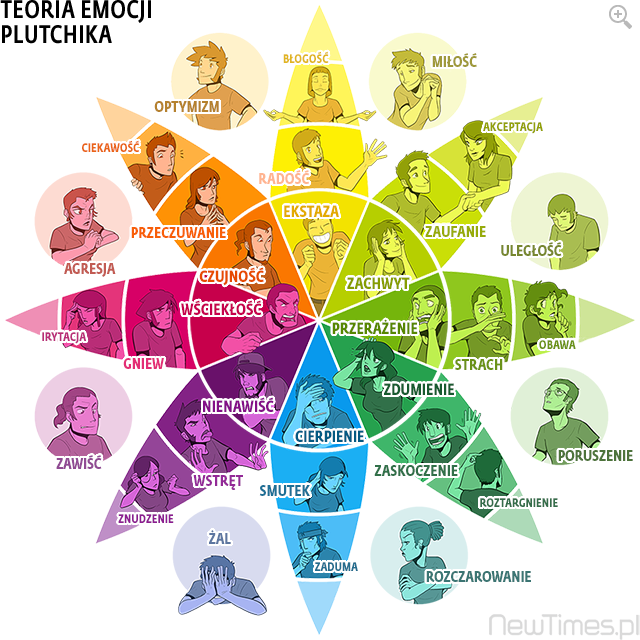
\includegraphics[height = 0.5\textwidth]{./plutchik}
  \end{figure}
\end{frame}
%%%%%%%%%%%%%%%%%%%%%%%%%%%%%%%%%%%%%%%%%%%%%%%%%%%%%%%%%%%%%%%%%%%%%%%%%%%%%%%%
\begin{frame}[t,fragile]{Wykorzystana baza danych}
\begin{itemize}
\item 12 mówców
\item zdania, polecenia, cyfry, tekst
\item 7 stanów emocjonalnych 
\item baza emocji odgrywanych
\end{itemize}
\end{frame}
%%%%%%%%%%%%%%%%%%%%%%%%%%%%%%%%%%%%%%%%%%%%%%%%%%%%%%%%%%%%%%%%%%%%%%%%%%%%%%%%
\begin{frame}[t,fragile]{Ekstrakcja cech, selekcja cech, kalifikacja}
\begin{itemize}
\item energia, entropia, MFCC, SSC, liczba przejść przez zero
\item statystyka
\item PCA, RFE
\item KNN, SVM, MLP
\end{itemize}
\end{frame}
%%%%%%%%%%%%%%%%%%%%%%%%%%%%%%%%%%%%%%%%%%%%%%%%%%%%%%%%%%%%%%%%%%%%%%%%%%%%%%%%
\begin{frame}[t,fragile]{Badanie, wyniki, wnioski}
Implementacja: Python, numpy scikit-learn

Zbadano rozróżnialność emocji dla 7 klas i parami dla różnych par reduktorów i klasyfikatorów

Dla 7 klas, MLP i PCA trafność 55,6\%.

Dla 2 klas wyróżniają się MLP lub SVM z PCA
\end{frame}
%%%%%%%%%%%%%%%%%%%%%%%%%%%%%%%%%%%%%%%%%%%%%%%%%%%%%%%%%%%%%%%%%%%%%%%%%%%%%%%%
\begin{frame}[t,fragile]{Badanie, wyniki, wnioski}
Rozróżniając parami, uzyskano 100\% trafności dla strachu i złości, radości i smutku, złości i smutku.
Trafność rozróżnienia pary  strach-zdziwienie < 70\%.
  \begin{figure}
   \centering
   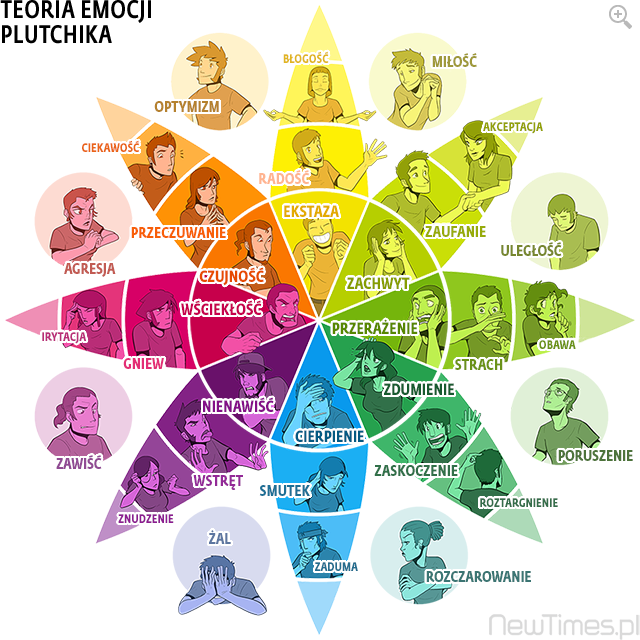
\includegraphics[height = 0.4\textwidth]{./plutchik}
  \end{figure}
\end{frame}
%%%%%%%%%%%%%%%%%%%%%%%%%%%%%%%%%%%%%%%%%%%%%%%%%%%%%%%%%%%%%%%%%%%%%%%%%%%%%%%%
\end{document}


